\documentclass[12pt]{article}
\usepackage{float}


\usepackage{amssymb,amsmath,amsthm}
\usepackage[top=1in, bottom=1in, left=1.25in, right=1.25in]{geometry}
\usepackage{fancyhdr}
\usepackage{mathtools}
\usepackage{enumerate}
\usepackage{color}
\usepackage[english]{babel}
\newtheorem*{theorem}{Theroem 7.12}
\newtheorem*{remark}{Remark}

%% Import a package useful for displaying graphics.
\usepackage{graphicx}

% Comment the following line to use TeX's default font of Computer Modern.
\usepackage{times,txfonts}

% Adjust line spacing an indentation
\parindent 0pt
\parskip 6pt plus 1pt

\newtheoremstyle{ex215}% name of the style to be used
  {18pt}% measure of space to leave above the theorem. E.g.: 3pt
  {12pt}% measure of space to leave below the theorem. E.g.: 3pt
  {}% name of font to use in the body of the theorem
  {}% measure of space to indent
  {\bfseries}% name of head font
  {:}% punctuation between head and body
  {2ex}% space after theorem head; " " = normal interword space
  {}% Manually specify head
\theoremstyle{ex215} 

\makeatletter
\newtheorem*{lemmacore}{Lemma \@currentlabel}
\newenvironment{lemma}[1]
{\def\@currentlabel{#1}\lemmacore}
{\endlemmacore}

\newtheorem*{corollarycore}{Corollary \@currentlabel}
\newenvironment{corollary}[1]
{\def\@currentlabel{#1}\corollarycore}
{\endcorollarycore}


%%%%%%%%%%%%%%%%%%%%%%%%%%%%%%%%%%%%%%%%%%%%%%%%%%%%%%%%%%%%%%%%%%%%%%%%
%
% Stuff for getting the name/document date/title across the header
\RequirePackage{fancyhdr}
\pagestyle{fancy}
\fancyfoot[C]{\ifnum \value{page} > 1\relax\thepage\fi}
\fancyhead[L]{\ifx\@doclabel\@empty\else\@doclabel\fi}
\fancyhead[C]{\ifx\@docauthor\@empty\else\@docdate\fi}
\fancyhead[R]{\ifx\@docauthor\@empty\@docdate\else\@docauthor\fi}
\headheight 15pt


\def\doclabel#1{\gdef\@doclabel{#1}}
\doclabel{Use {\tt\textbackslash doclabel\{MY LABEL\}}.}
\def\docdate#1{\gdef\@docdate{#1}}
\docdate{Use {\tt\textbackslash docdate\{MY DATE\}}.}
\def\docauthor#1{\gdef\@docauthor{#1}}
%\docauthor{Use {\tt\textbackslash docauthor\{MY NAME\}}.}
\let\@docauthor\@empty

\newcounter{probcount}
\newcounter{subprobcount}
\newlength\probsep
\newlength\pshrinking
\newif\iffirstprob

% The following commands allow for a handy override of labels in an enumeration,
% without having the user keep track of what level the enumeration is happening at.
% To use them, just put \listlabel{....} as the first command after a \begin{enumerate}.
% The '....' is used to define the label.  You can access the name of the current label
% counter with \thelistlabel.  Hence \listlabel{\textbf{\Alph{\thelistlabel}:}} would
% generate lists with bold labels A:, B:, C:, etc.
\newcommand{\listlabel}[1]{\def\thelistlabel{\@enumctr}%
            \expandafter\def\csname label\@enumctr\endcsname{#1}}


\newenvironment{subproblems}%
  {\begin{enumerate}\listlabel{\alph{\thelistlabel})}%
  %% Make the enumerate environment think we are making a list in a list:
  \global \@newlistfalse}%
  {\end{enumerate}}%

\newenvironment{problems}%
  {\ifhmode\unskip\par\fi\setcounter{probcount}{0}\probsep\parskip
  \sbox\@tempboxa{\textbf{9.}}\pshrinking\wd\@tempboxa\advance\pshrinking\labelsep
  \advance\linewidth -\pshrinking
  \advance\@totalleftmargin\pshrinking
  \advance\leftskip\pshrinking}%
  {\ifhmode\unskip \par\fi\advance\leftskip-\pshrinking}%

\newcommand{\problem}{%
  \setcounter{subprobcount}{0}%
  \stepcounter{probcount}%
  \def\@currentlabel{\arabic{probcount}}%
  \ifhmode
    \unskip \par
  \fi
%  \addpenalty{-4000}%
  \iffirstprob\else\addvspace\probsep\fi
  \firstprobfalse
  \hskip -\labelwidth\hskip -\labelsep 
  \hbox to\labelwidth{\hss\textbf{\arabic{probcount}.}}\hskip\labelsep
}%

%% The localhead command puts a label on top of a paragraph -- handy for labels
%% like "Solution:"
\newskip\restoreparskip
\newcommand{\localhead}[1]{\par\smallskip\textbf{#1}\nobreak\\}%
%% The following arcane code was added to make the localhead enviroment get along
%% with the ams theorem enviroment (which is based on the latex list enviroment).
%% previously, the command was {\par\smallskip\textbf{#1}\\}, but the list
%% enviroment would also add a par at the end of this paragraph, which would result
%% in an extra blank line.  Our solution now is to put in our own par, but with
%% none of the parskip glue that adds extra space between paragraphs.
%%  \restoreparskip\parskip\parskip 0pt\par\nobreak\noindent\parskip\restoreparskip}%
\newcommand\solution{\localhead{Solution:}}
\newcommand\subsol{\stepcounter{subprobcount}\localhead{Solution, part \alph{subprobcount}:}}
\newcommand\subsoleg[1]{\stepcounter{subprobcount}\par\textbf{Solution, part \alph{subprobcount}:} #1\\}
\def\solver#1{(Solution by #1)\\\vskip-12pt}


%% The default 'article' class has captions that label figures Figure 1, etc.  This is too 
%% formal for homework sets, so we change \caption so that it just puts the caption text.
%% Here I have just modified the \@makecaption command from the article class.
%% Maybe I should change this in the future to let authors decide whether or not to label a figure.

\long\def\@makecaption#1#2{%
  \vskip\abovecaptionskip
  \sbox\@tempboxa{#2}%
  \ifdim \wd\@tempboxa >\hsize
    #2\par
  \else
    \global \@minipagefalse
    \hb@xt@\hsize{\hfil\box\@tempboxa\hfil}%
  \fi
  \vskip\belowcaptionskip}

%% The default implementation of the proof environment starts a new paragraph at the start of the proof,
%% with the full parskip spacing. This only looks good following a theorem statement 
%% if \parskip is set to zero.  We've got a medium sized parskip, so we overide this 
%% questionable decision.
\renewenvironment{proof}[1][\proofname]{\par
  \pushQED{\qed}%
  \normalfont \topsep6\p@\@plus6\p@\relax
  \trivlist
  \@topsep \topsep
  \item[\hskip\labelsep
        \itshape
    #1\@addpunct{.}]\ignorespaces
}{%
  \popQED\endtrivlist\@endpefalse
}
\makeatother

% Shortcuts for blackboard bold number sets (reals, integers, etc.)
\newcommand{\Reals}{\ensuremath{\mathbb R}}
\newcommand{\Nats}{\ensuremath{\mathbb N}}
\newcommand{\Ints}{\ensuremath{\mathbb Z}}
\newcommand{\Rats}{\ensuremath{\mathbb Q}}
\newcommand{\Cplx}{\ensuremath{\mathbb C}}
\newcommand{\diam}[1]{\text{diam}(#1)}
\newcommand\converges[1]{\mathrel{\mathop{\longrightarrow}\limits_{#1}}}
\newcommand{\norm}[2]{\left \lVert #1 \right \rVert_{#2}}
\newcommand{\abs}[1]{\left| #1 \right|}


%% Some equivalents that some people may prefer.
\let\RR\Reals
\let\NN\Nats
\let\II\Ints
\let\CC\Cplx
\let\ZZ\Ints

\doclabel{Math F641: Take Home Midterm}
\docauthor{Stefano Fochesatto}
\docdate{\today}
\begin{document}
\begin{problems}



\problem Let $(a_n)$ and $(b_n)$ be sequences of numbers such that $a_n \leq b_n$ for all $n$. 
\begin{enumerate}
  \item[(a)] Give a carful proof that, 
  \begin{equation*}
    \limsup_{n \to \infty} a_n \leq \limsup_{n \to \infty} b_n
  \end{equation*}
  \begin{proof} Let $(a_n)$ and $(b_n)$ be sequences of numbers such that $a_n \leq b_n$ for all $n$. Now let $A_n = \sup\{a_n, a_{n + 1}, a_{n + 2}, \dots\}$ and $B_n =  \sup\{b_n, b_{n + 1}, b_{n + 2}, \dots\}$. Note that since $a_n \leq b_n$ for all $n$ it follows from the definition of the supremum that $A_n \leq B_n$ for all $n$. By the definition of $\limsup$ we know that, 
    \begin{equation*}
      \limsup_{n \to \infty} a_n = \inf_{n \geq 1}{A_n}, \qquad \limsup_{n \to \infty} b_n = \inf_{n \geq 1}{B_n}.
    \end{equation*}
    Since $A_n \leq B_n$ for all $n$ it must follows that 
    \begin{equation*}
      \limsup_{n \to \infty} a_n = \inf_{n \geq 1}{A_n} \leq \inf_{n \geq 1}{B_n} = \limsup_{n \to \infty} b_n.
    \end{equation*}

  \end{proof}




  \item[(b)] Show that it need not be true that 
  \begin{equation*}
    \limsup_{n \to \infty} a_n \leq \liminf_{n \to \infty} b_n
  \end{equation*}
  \solution Consider the following pair of sequences,
  \begin{equation*}
    b_n = (-1)^n \qquad a_n = \begin{cases}
      -\frac{1}{n}, \text{$n$ is odd}\\
      -1, \text{$n$ is even}
    \end{cases}
  \end{equation*}
  Note these sequences satisfy $a_n \leq b_n$ for all $n$ with the property that $\limsup_{n \to \infty} a_n = 0 > -1 = \liminf_{n \to \infty} b_n$. 
\end{enumerate}
\newpage


% Somewhat good
\problem \textbf{Carothers 8.53} Suppose that $f: \RR \to \RR$ is continuous and that $f(x) \to 0$ as $x \to \pm \infty$. Prove that $f$ is uniformly continuous. 
\begin{proof} Let $\epsilon > 0$. Since $f(x) \to 0$ as $x \to \pm \infty$ there exists a $K \in \RR$ such that for all $|x| \geq K$ we know that, 
  \begin{equation*}
    |f(x)| < \epsilon.
  \end{equation*}
  Now recall that $f|_{[-K, K]}$ is a continuous function on a compact interval, and therefore it must be uniformly continuous. Consider the appropriate $\delta> 0$ for our given $\epsilon$. To extend uniform continuity to all of $\RR$ without loss of generality consider $x \in [-K, K]$ and $|y|\geq K$, such that $|x - y| \leq \delta$
  \begin{align*}
    |f(x) - f(y)| &\leq |f(x) - f(K)| + |f(K) - f(y)| \\
    &\leq |f(x) - f(K)| + |f(K)- 0| + |0 - f(y)|< 3\epsilon.
  \end{align*}
  
\end{proof}
\newpage
 

\problem Determine if the following function are continuous. [You are welcome to use the Cauchy-Schwarz inequality for integrals].
\begin{enumerate}
  \item[(a)] $F: (C[0, 1], L^\infty) \to \RR$ defined by $F(f) = f(0)$. 
  \solution First we will demonstrate that $F$ is a linear operator. Let $f, g \in C[0, 1]$ and $\alpha, \beta \in \RR$,
  and note that, 
  \begin{equation*}
    F(\alpha f + \beta g) = \alpha f(0) + \beta g(0) = \alpha F(f) + \beta F(g). 
  \end{equation*} 
  Now to demonstrate continuity we will show that this linear operator is bounded.
  Let $f \in C[0, 1]$ and note that, 
  \begin{equation*}
    |F(f)|=|f(0)| \leq \max_{a \leq x \leq b} |f(x)| = \norm{f}{}.
  \end{equation*} 
  Thus $f$ is a bounded linear operator and is therefore continuous. 

  \item[(b)] $W: (C[0, 1], L^2) \to \RR$ defined by $W(f) = \int_0^1 f$.
  \solution Again we demonstrate that $W$ is a linear functional. Let $f, g \in (C[0, 1], L^2)$ and $\alpha, \beta \in \RR$,
  and note that, 
  \begin{equation*}
    W(\alpha f + \beta g) = \int_0^1 \alpha f(x) + \beta g(x) dx = \alpha \int_0^1f(x)dx + \beta \int_0^1g(x) dx = \alpha W(f) + \beta W(g). 
  \end{equation*} 
  Let $g(x)$ be a constant function with a value of 1 over $C[0,1]$ and by the Cauchy-Schwarz for integral we get the following, 
  \begin{align*}
    \abs{\int_0^1 f(x)dx} &= \left(\left(\int_0^1 f(x)dx\right)^2 \right)^{1/2} = \left(\left(\int_0^1 f(x)g(x)dx \right)^2 \right)^{1/2}\\ 
    &\leq \left(\int_0^1 f(x)^2 dx \int_0^1 g(x)^2dx\right)^{1/2} = \left(\int_0^1 f(x)^2 dx\right)^{1/2} = \norm{f}{2} \\
  \end{align*}
  Thus $W$ is a bounded linear map and is therefore continuous. 


  \item[(c)] $G: (C[0, 1], L^1) \to (C[0, 1], L^2)$ defined by $G(f) = f$
  \solution


  \item[(d)] $H: (C[0, 1], L^2) \to (C[0, 1], L^1)$ defined by $H(f) = f$
  \solution
  
\end{enumerate}
\newpage





% Clean up a little but mostly done. 
\problem \textbf{Carothers 10.20} $C^{(1)}[a, b]$ is the vector space of all functions $f: [a, b] \to \RR$ having a continuous first derivative on $[a, b]$. Show that $C^{(1)}[a, b]$ is complete under the norm $\norm{f}{C^{(1)}} = \max_{a \leq x \leq b} |f(x)| + \max_{a \leq x \leq b} |f'(x)|$. 
\begin{proof} Let $(f_n) \subseteq (C^{(1)}[a, b], \norm{\cdot}{C^{(1)}})$ be a Cauchy sequence of functions. Note that $(f_n') \subset C[a, b]$, and further note that since $f_n$ is Cauchy with respect to $\norm{\cdot}{C^{(1)}}$ it follows that for all $\epsilon > 0$ there exists an $N$ such that if $n, m \geq N$ we know that, 
  \begin{align*}
    \norm{f_n - f_m}{C^{(1)}} &=  \max_{a \leq x \leq b} |f_n(x) - f_m(x)| + \max_{a \leq x \leq b} |f_n'(x) - f_m'(x)|,\\
    &= \norm{f_n(x) - f_m(x)}{\infty} + \norm{f_n'(x) - f_m'(x)}{\infty},\\
    &< \epsilon. 
  \end{align*}
  Therefore an $N$ can be chosen to make, $\norm{f_n(x) - f_m(x)}{\infty}$ and $\norm{f_n'(x) - f_m'(x)}{\infty}$ arbitrarily small in $C[a, b]$ with respect to $L^\infty$. Therefore $(f_n)$ and $(f_n')$ are Cauchy in $C[a, b]$. Since $C[a, b]$ is complete there exists an $f, g \in C[a, b]$ such that $f_n \to f$ and $f_n' \to g$ uniformly with respect to $L^\infty$. It now follows by Theorem 10.7 that $f$ is a differentiable function on $[a, b]$, and that $f' = g$. Now we must show that $f_n \to f$ uniformly under $\norm{\cdot}{}$


  What is left to show is that $f \in C^{(1)}[a, b]$ and $f_n \to f$ with respect to $C^{(1)}[a, b]$. Let $\epsilon > 0$ and note that since $f_n \to f$ and $f_n' \to f'$ uniformly with respect to $L^\infty$ there exists an $N$ such that if $n \geq N$ then for all $x$, $ \norm{f_n(x) - f(x)}{\infty} < \epsilon$ and $\norm{f_n'(x) - f'(x)}{\infty} < \epsilon$ so it follows that, 
  \begin{align*}
    \norm{f_n - f}{C^{(1)}[a, b]} &=  \norm{f_n(x) - f(x)}{\infty} + \norm{f_n'(x) - f'(x)}{\infty}\\
    &< 2\epsilon. 
  \end{align*}


  
\end{proof}
\newpage







\problem \textbf{Carothers 10.33} Define $I(x) = 0$ for $x \leq 0$ and $I(x) = 1$ for $x > 0$. Given sequences $(x_n)$ and $(c_n)$ in $\RR$, with $\sum_{n = 1}^{\infty}|c_n| < \infty$, show that $f(x) = \sum_{n = 1}^\infty c_n I(x - x_n)$ defines a bounded function on $\RR$ that is continuous except, possibly at the $x_n$. 
\begin{proof} Let $\sum_{n = 1}^\infty |c_n| = M$ and note that for all $x \in \RR$ it follows that, 
  \begin{align*}
    |f(x)| &= \abs{\sum_{n = 1}^\infty c_n I(x - x_n)}\leq \abs{\sum_{n = 1}^\infty c_n} \leq \sum_{n = 1}^\infty \abs{c_n} = M.  
  \end{align*}
  Note that we have shown $f$ is a well-defined and bounded function. What is left to show is that $f$ is continuous on $\RR \setminus (x_n)$. 
  
  First let $x \in \RR\setminus (x_n)$, $\epsilon > 0$ and note that since  $\sum_{n = 1}^{\infty}|c_n| < \infty$ there exists an $N$ large enough such that  $\sum_{n = N + 1}^{\infty}|c_n| < \epsilon$, also note that each function $c_nI(x - x_n)$ is continuous at $x$, so there exists a $\delta_n$ such that
  when $0 < \abs{x - y} < \delta_n$, 
  it follows that, 
  \begin{equation*}
    \abs{c_n I(x - x_n) - c_n I(y - x_n)} < \epsilon. 
  \end{equation*}
  Considering $\delta = \min_{1 \leq n\leq N}\{\delta_n\}$ we find that when $0 < \abs{x - y} < \delta$,

  \begin{align*}
    \abs{f(x) - f(y)} &= \abs{\sum_{n = 1}^\infty c_n I(x - x_n) - \sum_{n = 1}^\infty c_n I(y - x_n)}\\
    &= \abs{\sum_{n = 1}^\infty c_n I(x - x_n) - c_n I(y - x_n)}\\
    &\leq \sum_{n = 1}^\infty \abs{c_n I(x - x_n) - c_n I(y - x_n)}\\
    &= \sum_{n = 1}^N \abs{c_n I(x - x_n) - c_n I(y - x_n)}+  \sum_{n = N + 1}^\infty \abs{c_n I(x - x_n) - c_n I(y - x_n)} < (N+1)\epsilon. 
  \end{align*}
\end{proof}
\newpage






\problem Let $X$ be a compact metric space, and let $\chi$ be the set of non-empty closed subsets of $X$. If $a \in X$ and $B \subseteq X$, we define $d(a, B) = \inf_{b \in B}d(a, b)$. We define a metric, called the Hausdorff distance, on $\chi$ by, 
\begin{equation*}
  H(A, B) = \sup_{a \in A}d(a, B) + \sup_{b \in B}d(b, A). 
\end{equation*}

\begin{enumerate}
  \item[(a)] Suppose $X \subseteq \RR^2$ is the closed ball of radius 100, $A$ is the closed square with side length 1 centered at the origin, and $B$ is the closed ball of radius 1/4 centered at the point (1/2, 1/2). Draw a picture of the arrangement and compute $H(A, B)$. (No rigor here please!)
  \solution
  \begin{figure}[H]
		\begin{center}
			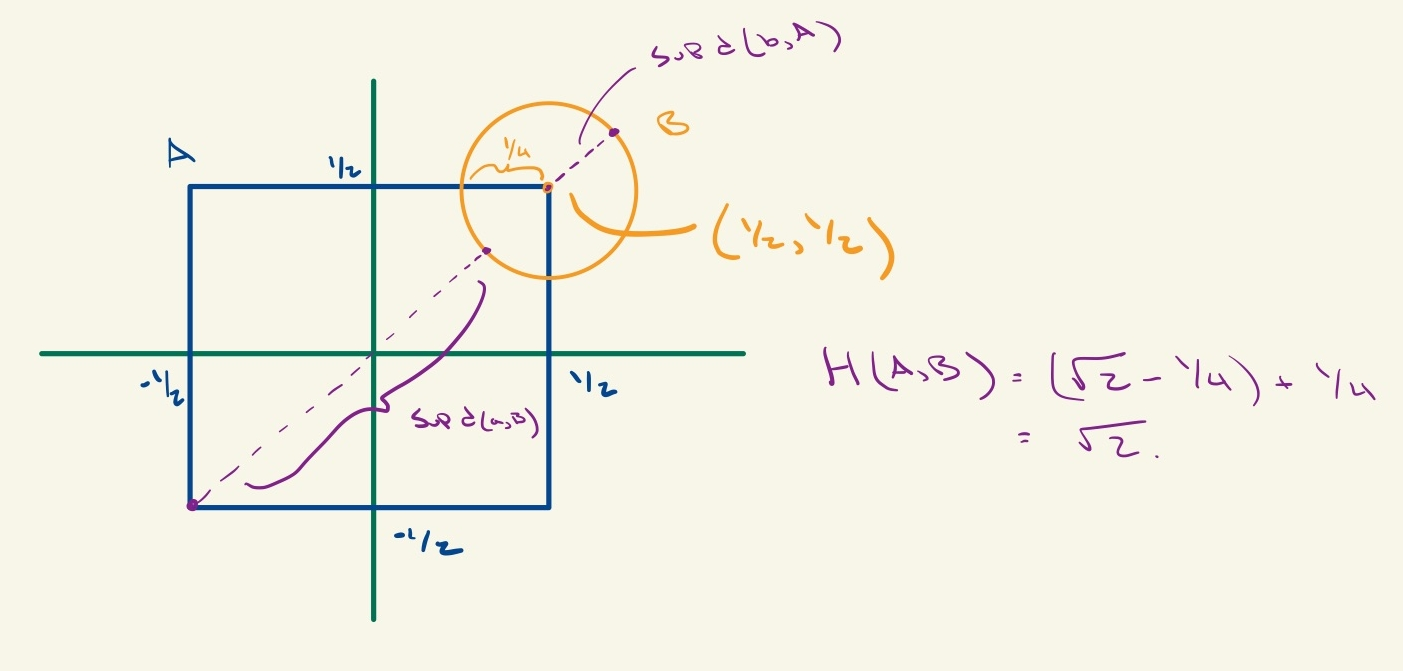
\includegraphics[width=.75\textwidth]{Hauss.jpg}
		\end{center}
	\end{figure}
  

  \item[(b)] Show that $H$ is a metric on $\chi$. 
  \begin{enumerate}
    \item $0 \leq H(A,B) < \infty$ for all pairs $A, B \in \chi$
    \begin{proof} This property is inherited from $X$ being a metric space. For a given pair of closed sets $A, B \in \chi$ we know that since $0 \leq d(b, a) < \infty$ for all $a, b \in X$,
      \begin{equation*}
        H(A, B) = \sup_{a \in A}\inf_{b \in B}d(a, b) + \sup_{b \in B}\inf_{a \in A}d(b, a) < \infty. 
      \end{equation*} 
    \end{proof}

    \item $H(A,B) = 0$ if and only if $A = B$
    \begin{proof} Suppose $A = B$, then clearly the set $\{d(a, B): a \in A\}$ is all zeros and similarly 
      with $\{d(b, A): b \in B\}$. So therefore,
      \begin{equation*}
        H(A, B) = \sup_{a \in A}d(a, B) + \sup_{b \in B}d(b, A) = 0
      \end{equation*}
    \end{proof}
    \begin{proof} Suppose $A \neq B$, then without loss of generality there exists some $x \in B$ such that $x \not\in A$. Now clearly $0 < \inf_{a \in A}d(x, a) \leq \sup_{b \in B}d(b, A)$ and therefore $H(A,B) \neq 0$
    \end{proof}

    \item $H(B,A) = H(A,B)$ for all $A,B \in \chi$,
    \begin{proof} Clearly this follows since, 
      \begin{equation*}
        H(A,B) = \sup_{a \in A}d(a, B) + \sup_{b \in B}d(b, A) =  \sup_{b \in B}d(b, A) + \sup_{a \in A}d(a, B) = H(B,A).
      \end{equation*}
    \end{proof}

    \item $H(A,B) \leq H(A,C) + H(C,B)$ for all $A, B, C \in \chi$. 
    \begin{proof} First note that since $X$ is a metric space it follows that, if we let $c \in C$ then for all $a \in A$ and $b \in B$, 
      \end{proof}
  \end{enumerate}
\end{enumerate}
\newpage




\problem Show that the previous space $\chi$ in the previous problem is totally bounded. 
\begin{proof} Let $X$ be a compact metric space, and let $\chi$ be the set of non-empty closed subsets of $X$. Let $\epsilon > 0$ and note that since $X$ is compact it is also totally bounded so there exists $\epsilon$-net with finitely many points $\{x_i\}_{i = 1}^N$ such that $X \subseteq  \cup_{i = 1}^N B_\epsilon(x_i)$.


  It is not clear to me how to write/ describe the $\epsilon$-net for $\chi$ from here. I know I want each point of the $\epsilon$-net for $\chi$ to look like a union of $\epsilon$-balls from my $\epsilon$-net of $X$. I want this since any point in $\chi$, is really a closed set in $X$ which can be covered within $\epsilon$-Hausdorff distance by a union of $\epsilon$-balls from my $\epsilon$-net of $X$. I guess what would be left to show is that the set of all such points for my proposed $\epsilon$-net for $\chi$ is finite, which would have to come from the fact that $\epsilon$-net for $X$ is finite. Then finally we would have that $\chi$ is totally bounded. 
 \end{proof}
\newpage





\problem Let $C^{2\pi}$ denote the continuous $2\pi$-periodic functions on $\RR$. Let $f \in C^{2\pi},$ and define
\begin{equation*}
  a_n = \frac{1}{\pi} \int_{-\pi}^{\pi} f(x)\cos(nx) dx, \qquad b_n = \frac{1}{\pi} \int_{-\pi}^{\pi} f(x)\sin(nx)dx.
\end{equation*}
for $n = 0, 1, 2, \dots$.

\begin{enumerate}
  \item[(a)] Suppose $h \in C^{2\pi}$ and, 
  \begin{equation*}
    \frac{1}{2\pi} \int_{-\pi}^\pi h(x) \cos(nx) dx = 0, \quad  \frac{1}{2\pi} \int_{-\pi}^\pi h(x) \sin(nx) dx = 0 \quad 
  \end{equation*}
  for $n = 0, 1, 2, \dots$ Show that $h = 0$. Hint: See Application 11.6
  \begin{proof} Since $h \in C^{2\pi}$, applying Weierstrass' Second Theorem, we know that there exists a sequence of trig polynomial $(T_n)$ such that $T_n \to h$ uniformly on $\RR$. Now note that $(h)(T_n) \to h^2$ uniformly on $\RR$. To see this let $\epsilon > 0$ and note that since $T_n \to h$ uniformly there exists an $N$ such that for all $n \geq N$ it follows that for all $x \in \RR$,
    \begin{equation*}
      |T_n(x) - h(x)| < \epsilon.
    \end{equation*}
      However since $h \in C^{2\pi}$, we know that $h$ is bounded so $\norm{h}{\infty} = M < \infty$ and therefore it also follows that for all $x \in \RR$,
    \begin{equation*}
      |h(x)T(x) - (h(x))^2| = |h(x)(T(x) - h(x))| = |h(x)||T_n(x) - h(x)| < M\epsilon. 
    \end{equation*} 
    Now since  $(h)(T_n) \to h^2$ uniformly on $\RR$ it also follows that 
    \begin{equation*}
      \frac{1}{2\pi}\int_{-\pi}^{\pi} h(x)T_n(x)dx = \frac{1}{2\pi}\int_{-\pi}^{\pi} h^2(x)dx
    \end{equation*}
    Note that we can define $T_n(x)$ by some pair of sequences of real numbers $a_n$ and $b_n$
    where,
    \begin{equation*}
      T(x) = \sum_{k = 0}^n\left(a_k \cos(kx) + b_k\sin(kx)\right).
    \end{equation*}
    By substitution we get the following, 
      \begin{multline*}  
        \frac{1}{2\pi}\int_{-\pi}^{\pi} h(x)\left(\sum_{k = 0}^n\left(a_k \cos(kx) + b_k\sin(kx)\right)\right)dx=\\  \frac{1}{2\pi}\int_{-\pi}^{\pi} \sum_{k = 0}^n\left(a_k h(x)\cos(kx) + b_kh(x)\sin(kx)\right)dx
      \end{multline*}
      and by linearity of the integral it follows that, 
      \begin{multline*}
        \frac{1}{2\pi}\int_{-\pi}^{\pi} h(x)T_n(x)dx = \frac{1}{2\pi}\int_{-\pi}^{\pi}\sum_{k = 1}^n\left(a_k h(x)\cos(kx) + b_kh(x)\sin(kx)\right)dx =\\
        \sum_{k = 1}^n a_k \left(\frac{1}{2\pi}\int_{-\pi}^{\pi} h(x)\cos(kx)dx \right) + b_k\left(\frac{1}{2\pi}\int_{-\pi}^{\pi} h(x)\sin(kx)dx\right)=0
      \end{multline*}
      Thus it follows that, 
      \begin{equation*}
        \frac{1}{2\pi}\int_{-\pi}^{\pi} h^2(x)dx = 0.
      \end{equation*}
      Since $h$ is continuous, non-zero function values are forced to contribute to the size of integral and since the integral of $h^2$ on $[-\pi, \pi]$ is 0 it must be the case that $h(x) = 0$ on $[-\pi, \pi]$ and since $h \in C^{2\pi}$ we know that $h(x) = 0$ on $\RR$.
    






  \end{proof}
    







  \item[(b)] Suppose that $\sum_{n = 1}^\infty |a_n| + |b_n|$ converges. Show that the series
  \begin{equation*}
    \frac{a_0}{2} + \sum_{n = 1}^\infty a_n\cos(nx) + b_n\sin(nx)
  \end{equation*} 
  converges uniformly to a function $g \in C^{2n}$. 
  \begin{proof} First let, 
    \begin{equation*}
      g_n(x) = \frac{a_0}{2} + \sum_{k = 1}^n a_k\cos(kx) + b_k\sin(kx)
    \end{equation*}
    Note each $g_n$ is well-defined, since for a fixed $x \in \RR$, 
    \begin{align*}
      g_n(x) &\leq \abs{\frac{a_0}{2} + \sum_{k = 1}^n a_k\cos(kx) + b_k\sin(kx)},\\
      &\leq \abs{\frac{a_0}{2}} + \abs{\sum_{k = 1}^n a_k\cos(kx) + b_k\sin(kx)},\\
      &\leq \abs{\frac{a_0}{2}} + \sum_{k = 1}^n \abs{a_k}\abs{\cos(kx)} + \abs{b_k}\abs{\sin(kx)},\\
      &\leq \abs{\frac{a_0}{2}} + \sum_{k = 1}^n \abs{a_k} + \abs{b_k} < \infty. \\
    \end{align*}

      Let $g$ be the pointwise limit of $g_n$, which is also well defined since for a fixed $x \in \RR$, 
    \begin{align*}
      g(x) &\leq \abs{\frac{a_0}{2} + \sum_{n = 1}^\infty a_n\cos(nx) + b_n\sin(nx)},\\
      &\leq \abs{\frac{a_0}{2}} + \abs{\sum_{n = 1}^\infty a_n\cos(nx) + b_n\sin(nx)},\\
      &\leq \abs{\frac{a_0}{2}} + \sum_{n = 1}^\infty \abs{a_n}\abs{\cos(nx)} + \abs{b_n}\abs{\sin(nx)},\\
      &\leq \abs{\frac{a_0}{2}} + \sum_{n = 1}^\infty \abs{a_n} + \abs{b_n} < \infty. \\
    \end{align*}
    Note that since each $g_n \in C^{2\pi}$ we get that,
    \begin{equation*}
      g(-\pi) = \lim_{n \to \infty}g_n(-\pi) = \lim_{n \to \infty} g_n(\pi) = g(\pi),
    \end{equation*} 
      So we find that $g \in C^{2\pi}$. Now what is left to show is that $g_n \to g$ uniformly on $\RR$. Let $\epsilon > 0$ and choose $N$ such that $\sum_{k = N}^\infty |a_k| + |b_k| < \epsilon$ and note that for all $n \geq N$ and all $x \in \RR$  it follows that, 
    \begin{align*}
      \abs{g_n(x) - g(x)} &= \abs{\left(\frac{a_0}{2} + \sum_{k = 1}^n a_k\cos(kx) + b_k\sin(kx)\right) - \left(\frac{a_0}{2} + \sum_{k = 1}^\infty a_k\cos(kx) + b_k\sin(kx)\right)}\\
      &=\abs{\sum_{k = n + 1}^\infty a_k\cos(kx) + b_k\sin(kx)} \\
      &\leq \sum_{k = n + 1}^\infty \abs{a_k\cos(kx) + b_k\sin(kx)}\\
      &\leq \sum_{k = n + 1}^\infty \abs{a_k}\abs{\cos(kx)} + \abs{b_k}\abs{\sin(kx)}\\
      &\leq \sum_{k = n + 1}^\infty \abs{a_k} + \abs{b_k} \leq \epsilon
    \end{align*}
  \end{proof}






  \item[(c)] Recall the function $g$ just defined. Let 
  \begin{equation*}
    \hat{a}_n = \frac{1}{\pi}\int_{-\pi}^{\pi} g(x) \cos(nx) dx, \quad \hat{b}_n = \frac{1}{\pi}\int_{-\pi}^{\pi} g(x) \sin(nx) dx.
  \end{equation*}
  Show that $a_n = \hat{a}_n$, and $b_n = \hat{b}_n$ for all $n$. 
  \begin{proof} We will begin by demonstrating $a_n = \hat{a}_n$ noting that by a similar argument we can also conclude that $b_n = \hat{b}_n$. Recall $g_n(x)$ and define the following, 
    \begin{equation*}
      \hat{a}_{n, N} = \frac{1}{\pi}\int_{-\pi}^{\pi} g_N(x) \cos(nx) dx.
    \end{equation*} 
    First we will demonstrate that whenever $N \geq n$ it is the case that $\hat{a}_{n, N} = a_n$ and then we will demonstrate that $\lim_{N \to \infty} \hat{a}_{n, N} = \hat{a}_n$ which will then allow us to conclude that $\hat{a}_n = a_n$.
    
    Now consider the following expansion of $\hat{a}_{n, N}$ by the linearity of the integral, 
    \begin{equation*}
      \hat{a}_{n, N} = \frac{1}{\pi} \left(\frac{a_0}{2}\int_{-\pi}^{\pi} \cos(nx)dx + \sum_{k = 1}^N \left(a_k\int_{-\pi}^{\pi} \cos(kx)\cos(nx) dx\right) + \sum_{k = 1}^N\left(b_k\int_{-\pi}^{\pi} \sin(kx)\cos(nx)dx\right)\right)
    \end{equation*}
    We will proceed with an understanding that integrals of the following forms where $m \in \ZZ$, evaluate to zero, 
    \begin{equation*}
      \int_{-\pi}^{\pi}\sin(mx)dx = \frac{1}{m}[-\cos(m\pi)+\cos(-m\pi)] = \frac{1}{m}[-\cos(m\pi)+\cos(m\pi)] = 0.
    \end{equation*}
    \begin{equation*}
      \int_{-\pi}^{\pi}\cos(mx)dx = \frac{1}{m}[\sin(m\pi)-\sin(-m\pi)] = \frac{1}{m}[0] = 0.
    \end{equation*}
    Now consider that when $k \neq n$ we get the following by the angle sum identities, 
    \begin{align*}
      a_k\int_{-\pi}^{\pi} \cos(kx)\cos(nx) dx &= \frac{a_k}{2}\int_{-\pi}^{\pi} \cos((k+n)x) + \cos((k - n)x) dx \\
      &=\frac{a_k}{2}\left(\int_{-\pi}^{\pi} \cos((k+n)x)dx + \int_{-\pi}^{\pi}\cos((k - n)x) dx\right) \\
      &= \frac{a_k}{2}\left(0\right) = 0,
    \end{align*}
    \begin{align*}
      b_k\int_{-\pi}^{\pi} \sin(kx)\cos(nx)dx &= \frac{b_k}{2} \int_{-\pi}^{\pi} \sin((k + n)x) + \sin((k - n)x)dx\\
      &=\frac{b_k}{2} \left(\int_{-\pi}^{\pi} \sin((k + n)x)dx + \int_{-\pi}^{\pi}\sin((k - n)x)dx\right)\\
      &= \frac{b_k}{2}\left(0\right) = 0.
    \end{align*}
    Now when $k = n$, we get the following by the half-angle identity, 
    \begin{align*}
      a_n\int_{-\pi}^{\pi} \cos^2(nx) dx &= \frac{a_k}{2}\int_{-\pi}^{\pi} 1 + \cos(2nx),\\
      &= \frac{a_n}{2}\left(\int_{-\pi}^{\pi} 1 + \int_{-\pi}^{\pi}\cos(2nx)\right),\\
      &= \frac{a_n}{2}\left(2\pi\right),\\
      &= a_n\pi.
    \end{align*} 
    Applying the angle sum identities again we also find that,
    \begin{equation*}
      b_n \int_{-\pi}^{\pi} \sin(nx)\cos(nx)dx = \frac{b_n}{2}\int_{-\pi}^{\pi} \sin(2nx)dx =   \frac{b_n}{2}(0) = 0.
    \end{equation*}
    Putting our findings together we get that whenever $N \geq n$ it follows that, 
    \begin{equation*}
      \hat{a}_{n, N} = \frac{1}{\pi}\left(a_n\pi\right) = a_n. 
    \end{equation*}
    Now we must show that $\lim_{N \to \infty}\hat{a}_{n, N} = \hat{a}_n$. Let $\epsilon > 0$ and recall that $g_n \to g$ uniformly and therefore there exists an $M$ such that for all $n \geq M$ and $x \in \RR$ we know that, 
    \begin{equation*}
      \abs{g_n(x) - g(x)} = \abs{\sum_{k = n + 1}^\infty a_k\cos(kx) + b_k\sin(kx)} < \epsilon
    \end{equation*}
    so consider $N \geq M$ and we can conclude that, 
    \begin{align*}
      \abs{\hat{a}_{n, N} - \hat{a}_{n} } &= \abs{\frac{1}{\pi}\int_{-\pi}^{\pi} g_N(x) \cos(nx) dx - \frac{1}{\pi}\int_{-\pi}^{\pi} g(x) \cos(nx) dx}\\
      &= \abs{\frac{1}{\pi}\int_{-\pi}^{\pi} \left(g_N(x) - g(x)\right) \cos(nx) dx}\\
      &\leq \abs{\frac{1}{\pi}}\int_{-\pi}^{\pi} \abs{g_N(x) - g(x)} \abs{\cos(nx)}dx\\
      &< \abs{\frac{1}{\pi}}\int_{-\pi}^{\pi} \epsilon dx\\
      &= \abs{\frac{1}{\pi}}{2\pi}\epsilon\\
      &= 2\epsilon
    \end{align*}
    Therefore $\hat{a}_n =a_n$ for all $n$. 
  \end{proof}


  \item[(d)] Conclude that $f = g$. 

  \begin{proof} First note that if $\hat{a}_n = a_n$ for all $n$ it also follows that $\hat{a}_{n} - a_n = 0$ for all $n$, and analogously for $\hat{b}_{n}$ and $b_n$. Now applying this identity we can conclude that, 
    \begin{equation*}
      \frac{1}{2\pi}\int_{-\pi}^{\pi} (g(x)-f(x)) \cos(nx) dx = 0, \quad \frac{1}{2\pi}\int_{-\pi}^{\pi} (g(x)-f(x)) \sin(nx) dx = 0
    \end{equation*}
    By part a) we can conclude that $g(x) - f(x) = 0$ for all $x \in \RR$ and therefore $g(x) = f(x)$.
   \end{proof}




\end{enumerate}

\begin{remark}  
 In this problem you've shown that each element of $C^{2\pi}$ determines a different
collection of numbers $(a_n)$ and $(b_n)$. Moreover, if these sequences converge to zero so
fast that the series in part 2 converges, then the Fourier series of f converges uniformly
to $f$. This begs the question: given an arbitrary element of $C^{2\pi}$, is it true that the series in part 2 converges? This is food for thought, not food for the exam.
\end{remark}
\newpage



% To show $f$ is differentiable we need 


%$f_n \to f$ where each $f_n$ is cts and differentiable on $\RR$. 
% each $f'_n$ is continuous on $\RR$
% $f'_n \to g$ uniformly for some $g$. 
% f_n(x_0) \to c for some $c \in \RR$ and $x_0 \in \RR$. 



\problem Suppose $\sum|a_n|$ converges. By Carothers Exercise 10.26 we can define a function $f \in C(\RR)$ by $f(x) = \sum_{n = 0}^\infty a_n \sin(nx)$. 
\begin{enumerate}
  \item[(a)] If there exists constants $M > 0$ and $\alpha > 2$ such $|a_n| \leq \frac{M}{n^\alpha}$, prove that $f$ is differentiable.
  \begin{proof} Recall the statement of Exercise 10.26 which states that if $\sum_{n = 1}^\infty \abs{a_n}< \infty$, then $\sum_{n = 1}^\infty a_n \sin(nx)$ and $\sum_{n = 1}^\infty a_n \cos(nx)$ are uniformly convergent on $\RR$. Define the following, 
    \begin{equation*}
      f_n(x) = \sum_{k = 1}^n a_k \sin(kx)
    \end{equation*}
    and by Exercise 10.26 we know that $f_n \to f$ converges uniformly. We will proceed to show that $f$ is differentiable by applying Theorem 10.7. First we must show that each $f_n$ is continuous and differentiable on $\RR$. Clearly this is the case as each $f_n$ is a finite sum of continuous and differentiable functions on $\RR$. Now we must show that each $f'_n$ is continuous on $\RR$. Note that 
    \begin{equation*}
      f'_n(x) = \sum_{k = 1}^n a_k\cos(kx)(k),
    \end{equation*}
    which is a finite sum of continuous functions, so clearly each $f'_n$ is also continuous on $\RR$. Now we must show that $f'_n \to g$ uniformly on $\RR$, or equivalently that $\sum_{k = 1}^\infty a_k\cos(kx)(k)$ converges uniformly. Let $M_n = \frac{M}{n^{\alpha-1}}$ and it follows by our hypothesis that for all $x \in \RR$, 
    \begin{equation*}
      |a_n\cos(nx)(n)| \leq |a_n||\cos(nx)|n \leq |a_n|n \leq \frac{M}{n^\alpha}n = M_n
    \end{equation*}
    Note that since $\alpha \geq 3$ we know that $\alpha - 1 \geq 2$ and therefore, 
    \begin{equation*}
      \sum_{n = 1}^\infty M_n = \sum_{n = 1}^\infty \frac{M}{n^{\alpha-1}} = M\sum_{n = 1}^\infty \frac{1}{n^{\alpha-1}} 
    \end{equation*}
    is bounded above by a convergent $p$-series and therefore by the Weirstrass $M$-test, $\sum_{k = 1}^\infty a_k\cos(kx)(k)$ converges uniformly.
    Applying Theorem 10.7 we can conclude that $f$ is differentiable on $\RR$. 

  \end{proof}

  \item[(b)] Visit http://mathworld.wolfram.com/FourierSeriesTriangleWave.html.
  Then remark on what that has to do with the current problem.
  \solution The Fourier series for a symmetric triangle wave with period $2L$ is given by,
  \begin{equation*}
    f(x) = \dfrac{8}{\pi^2}
    \sum_{n = 1, 3, 5\dots}^\infty \dfrac{(-1)^{(n - 1)/2}}{n^2} \sin\left(\dfrac{n\pi x}{L}\right)
  \end{equation*}
  Applying what we've shown in part a) there is a sense that $f'$ is relatively well behaved since the fourier coefficients of $f$ converge, 
  \begin{equation*}
    \dfrac{8}{\pi^2}\sum_{n = 1, 3, 5\dots}^\infty \abs{\dfrac{(-1)^{(n - 1)/2}}{n^2}} \leq \dfrac{8}{\pi^2}\sum_{n = 1, 3, 5\dots}^\infty \abs{\dfrac{1}{n^2}} < \infty. 
  \end{equation*}
  Now, in the examples illustrated in the article with the asymmetric triangle wave we see that derivative of the first $(1/m)th$ and last $(1/m)th$ distance on the $2L$ interval are increasing/decreasing towards $\pm \infty$. We see this represented in the equation for the fourier coefficients of these asymmetric triangle waves, 
  We note that as we increase $m$ the series of fourier coefficients converge slower. 
  

\end{enumerate}

\begin{remark}
This problem illustrates a special case of the general principle that the faster the
Fourier coefficients of a function converge to zero, the smoother that function is.
2
\end{remark}



\end{problems}
\end{document}
